\documentclass[a4paper]{article}

\usepackage[english]{babel}
\usepackage{amsmath}
\usepackage{amssymb}
\usepackage{dsfont}
\usepackage{tikz}
\usepackage{framed} 
\usetikzlibrary{arrows,automata}
\title{Calculus and Probability Theory\\ Assignment 3}
\author{Christoph Schmidl\\
s4226887\\
Informatica\\
c.schmidl@student.ru.nl\\}
\date{\today}


\begin{document}
\maketitle

\textbf{After completing these exercises successfully you should be confident with the following topics:}

\begin{itemize}
	\item Apply all differentiation rules on elementary and transcendental functions 
	\item Solve problems including higher-order derivatives
	\item Apply l'Hopital's rules when applicable
	\item analyse graphs of a given real function
\end{itemize}
\vspace{1em}

\begin{enumerate}

\item (\textbf{10 points}) The function arcsin is the inverse function of sin.

\begin{enumerate}
	\item What is the domain of the function $\arcsin(x)$? Why?\\
	\textbf{Solution:}\\
	
\begin{figure}[ht]
  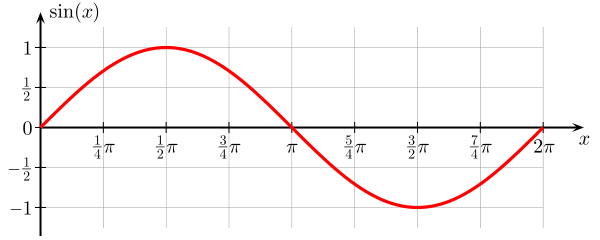
\includegraphics[width=0.6\textwidth]{sine.png}
  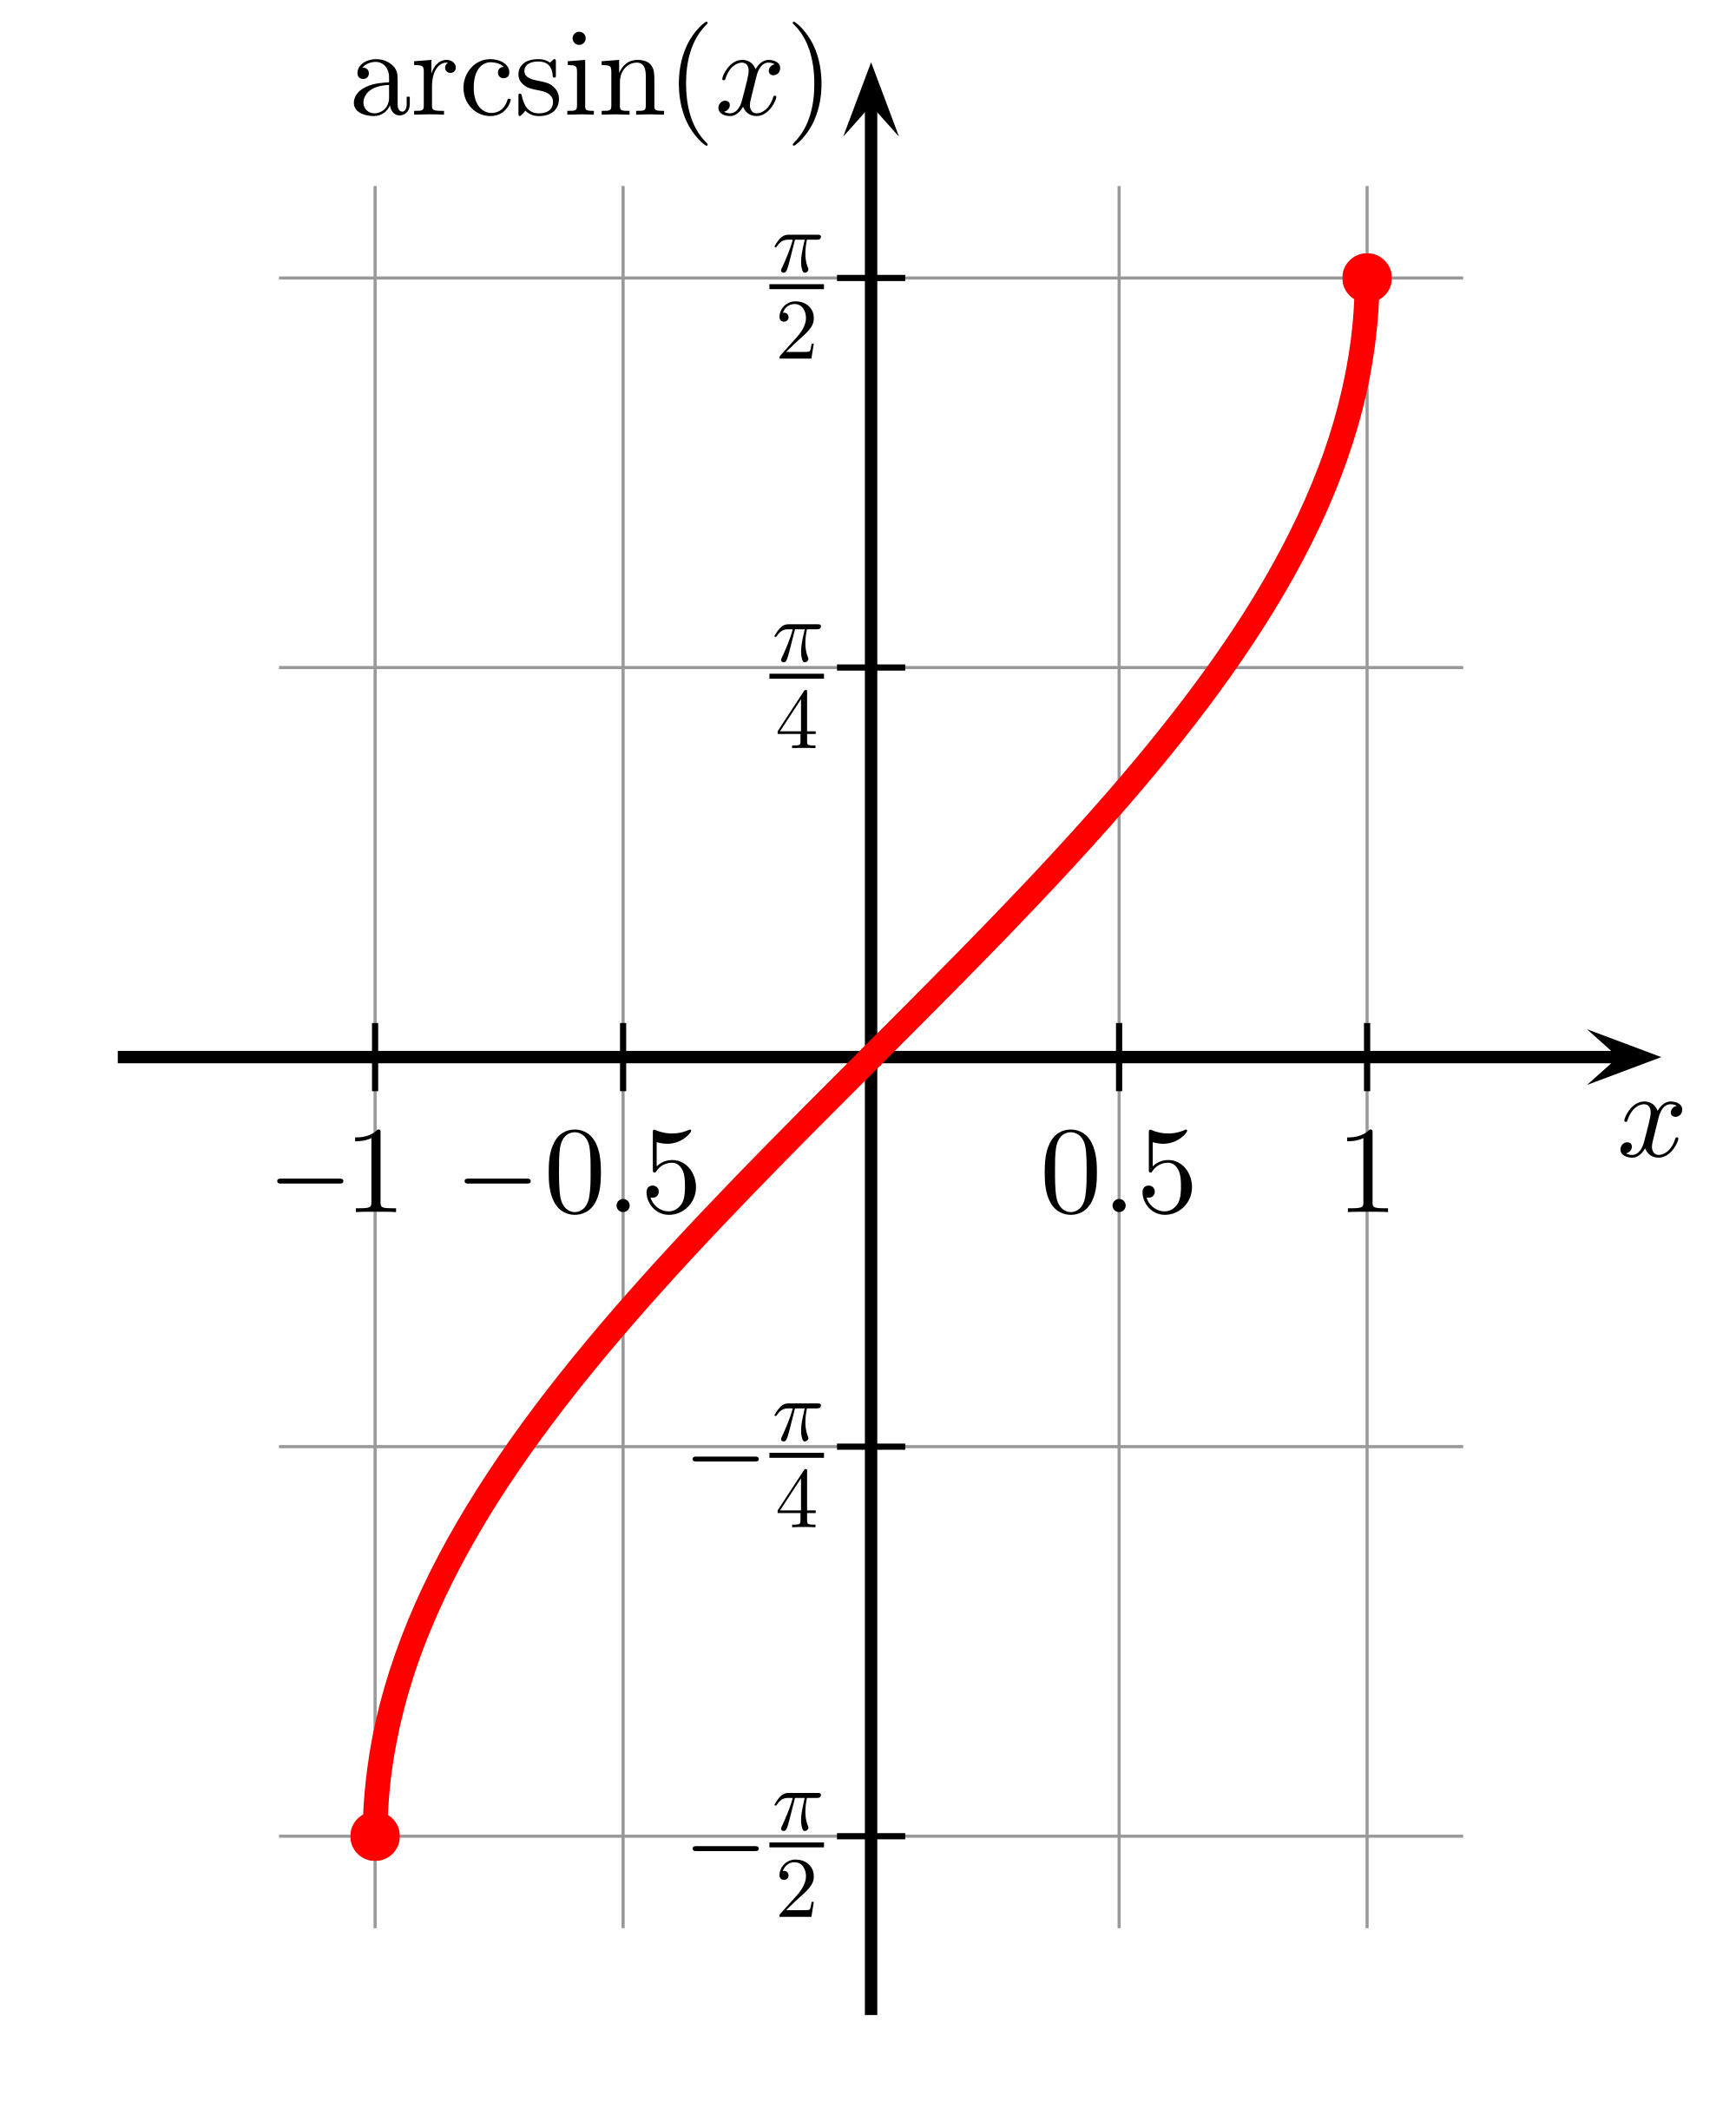
\includegraphics[width=0.3\textwidth]{arcsine.png}
\end{figure}	
	
	
As we already know, the domain of $\sin$ is $\mathbb{R}$ and its range is $[-1,1]$. Because $\arcsin$ is the inverse function of $\sin$ and reverses the output of $\sin$, the domain of $\arcsin$ is the range of $\sin$. Therefore, the domain of $\arcsin$ is $[-1,1]$.
	

\newpage

	
	
	\item Compute the following values and explain how you got the result:\\
	
\begin{figure}[ht!]
	\centering
  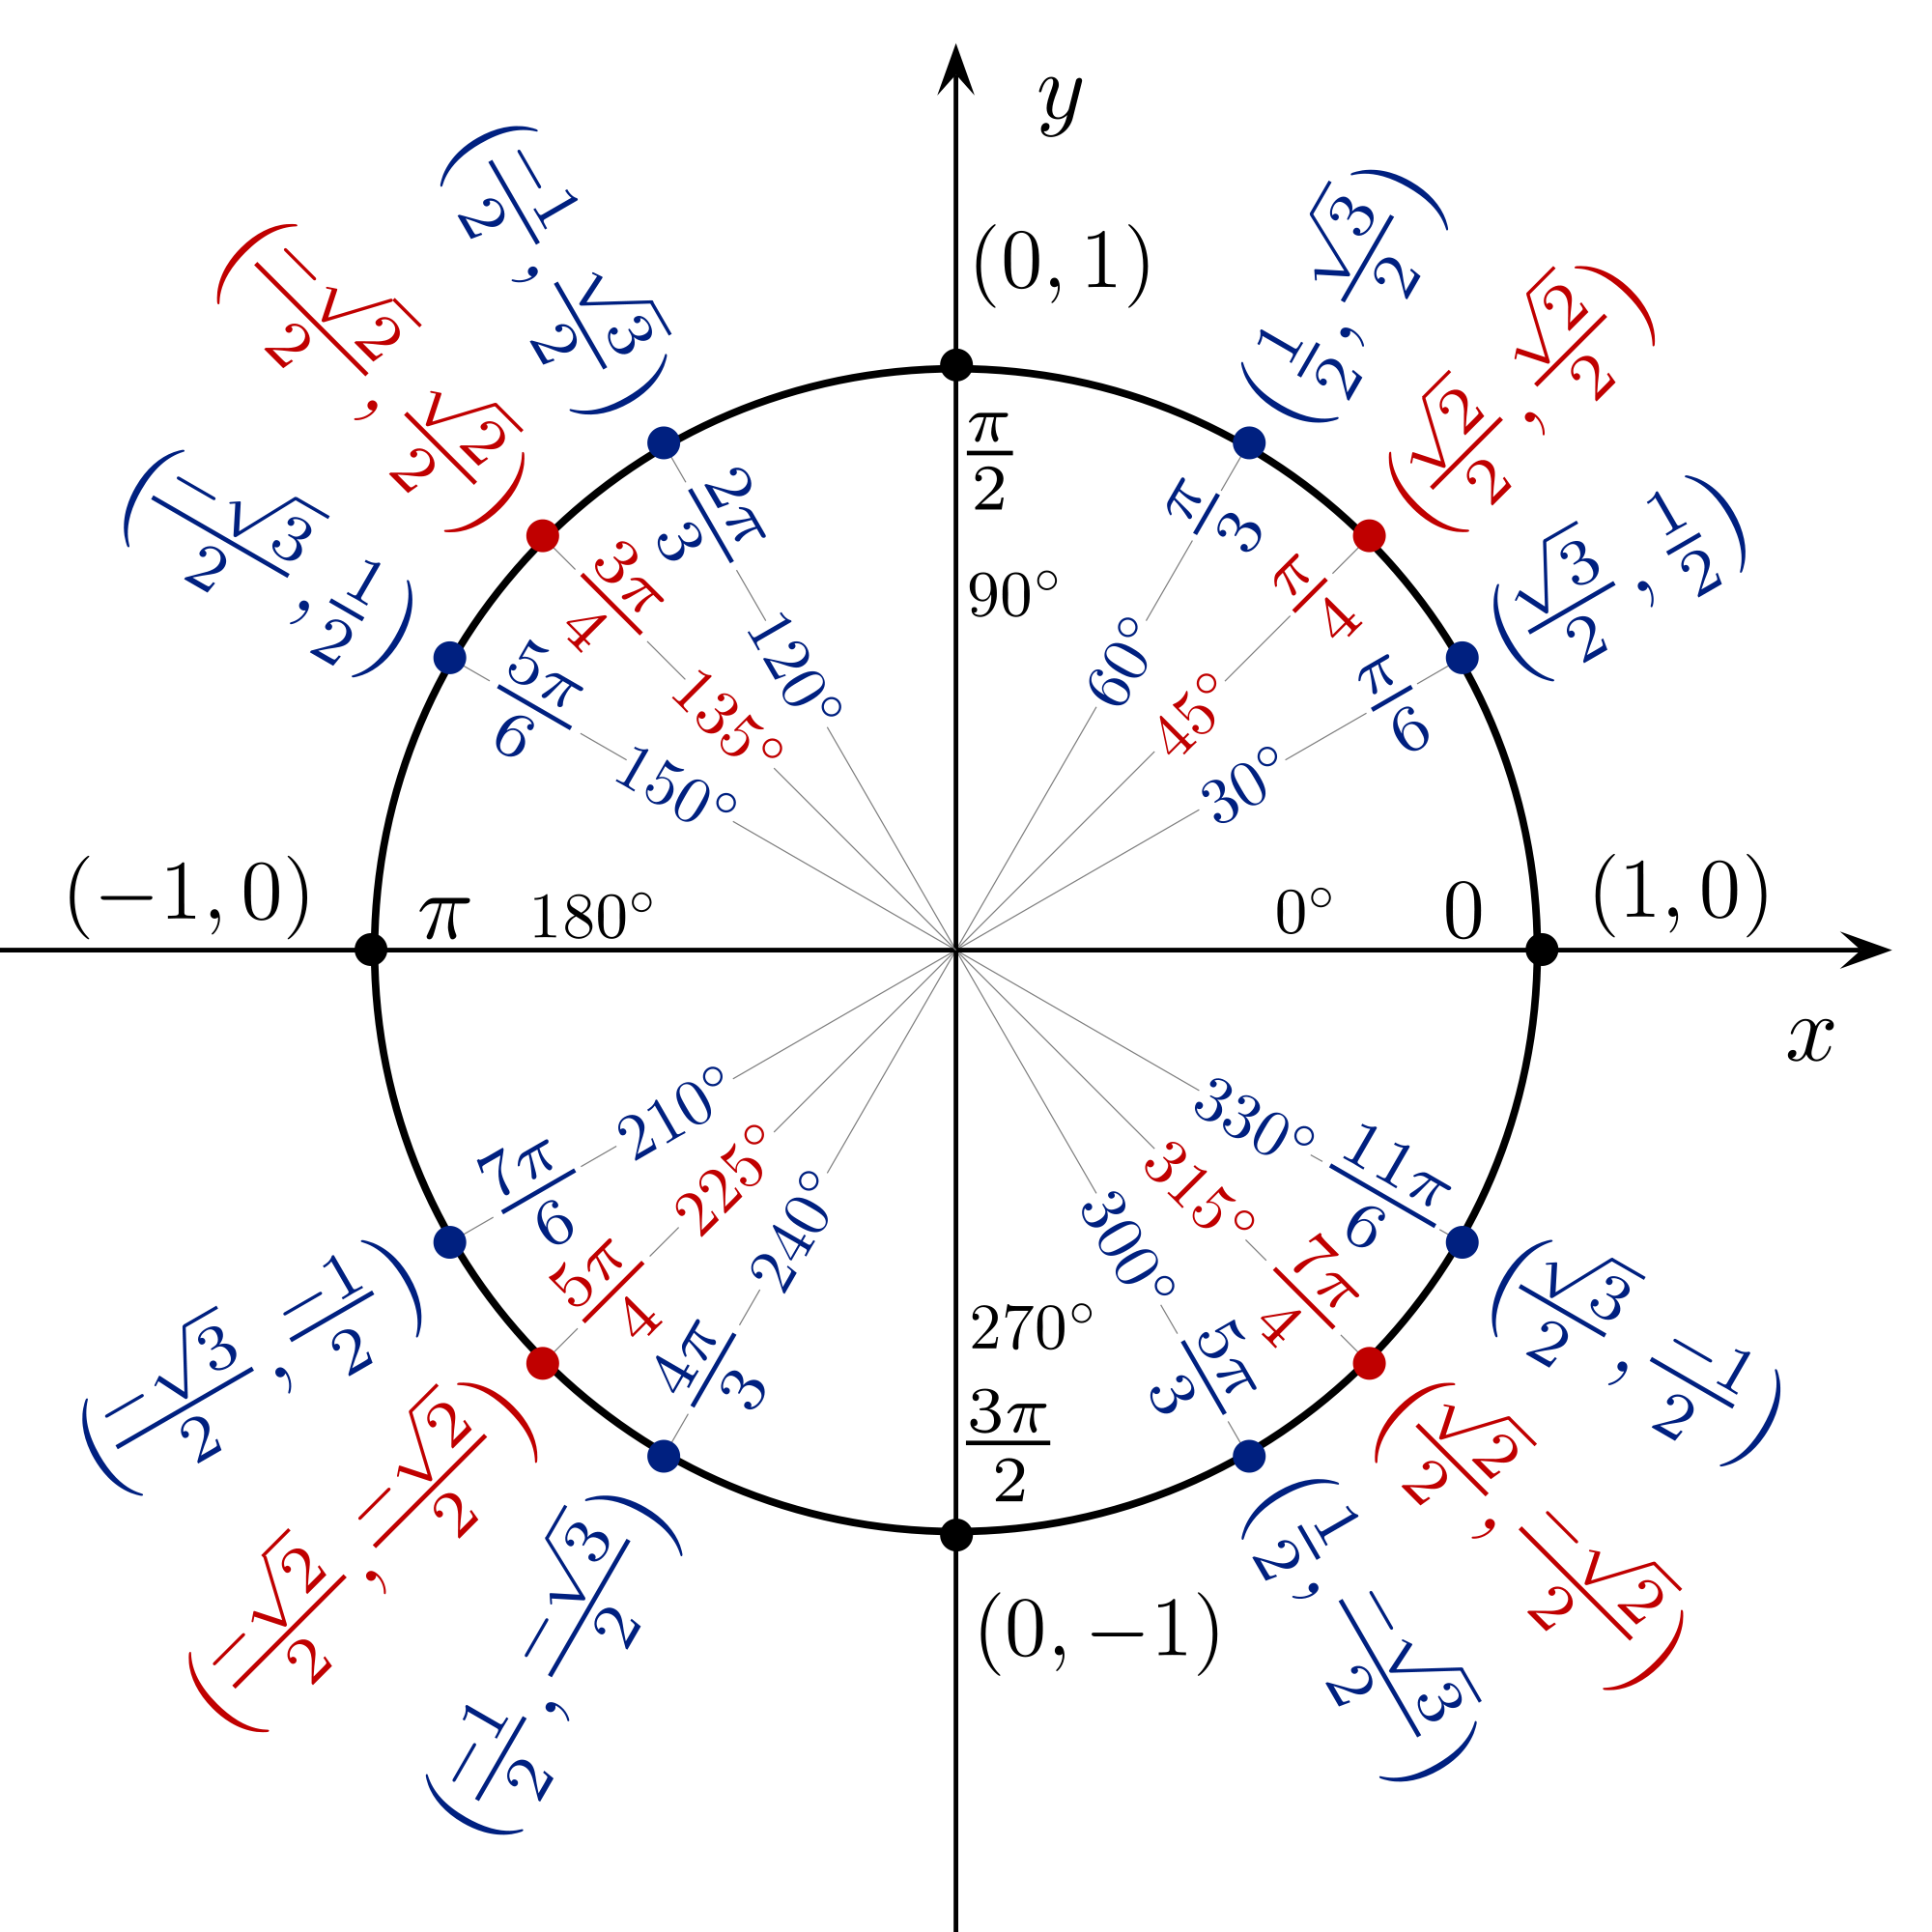
\includegraphics[width=0.7\textwidth]{unitcircle.png}
\end{figure}	

	
\begin{itemize}
	\item 	$\arcsin(1) = ?$\\
	\textbf{Solution:}\\
	
	
This can be rewritten as: What angle would I have to take the $sine$ of in order to get $1$? 
$\rightarrow \sin(?) = 1$\\
The answer is $\arcsin(1) = \frac{\pi}{2}$, because I know (by remembering the Unit Circle and the Sine function) that $\sin(\frac{\pi}{2}) = 1$.\\

	\item 	$\arcsin(0) = ?$\\
	\textbf{Solution:}\\
	
This can be rewritten as: What angle would I have to take the $sine$ of in order to get $0$?
$\rightarrow \sin(?) = 0$\\	

The problem is that $\arcsin(x)$ is NOT the true inverse of $\sin(x)$. In fact, $\sin(x)$ doesn't have an inverse function since it fails the horizontal line test. $\arcsin(x)$ is actually just the inverse of $\sin(x)$ on the interval $[-\pi/2, \pi/2]$ (the only interval where $\sin(x)$ is strictly increasing that contains the origin).\\ 

Thus, the value of $\arcsin(0)$ is the value of $x$ on the interval $[\piπ/2, \pi/2]$ that satisfies $\sin(x) = 0$. The only value of $x$ on $[-\pi/2, \pi/2]$ that does this is $x = 0$, so: 
$\arcsin(0) = 0$.\\ 


	\item 	$\arcsin(\frac{\sqrt{3}}{2}) = ?$\\
	\textbf{Solution:}\\	
	
By remembering the Unit Circle, I know that $\sin(\frac{\pi}{3}) = \frac{\sqrt{3}}{2}$. Therefore, $\arcsin\frac{\sqrt{3}}{2} = \frac{\pi}{3}$.\\	
	

This can be rewritten as: What angle would I have to take the $sine$ of in order to get $\frac{\sqrt{3}}{2}$?
$\rightarrow \sin(?) = \frac{\sqrt{3}}{2}$\\


\end{itemize}	
	

	

	



	\item Find the derivative of $f$:
	
	\begin{align*}
		f(x) = \arcsin(\frac{2x}{1-x})\notag
	\end{align*}
\textbf{Solution:}\\

Using chainrule with quotientrule.\\

\begin{align*}
	y &= \arcsin(x)\notag\\
	\sin(y) &= x\notag\\
	(\cos(y) \cdot y') &= 1\notag\\
	y' &= \frac{1}{\cos(y)}\notag\\
	\cos^2(y) + \sin^2(y) &= 1\notag\\
	\cos^2(y) &= 1 - \sin^2(y)\notag\\
	\cos(y) &= \sqrt{1 - \sin^2(y)}\notag\\
	y' &= \frac{1}{\cos(y)}\notag\\
	&= \frac{1}{\sqrt{1 - \sin^2(y)}}\notag\\
	&= \frac{1}{\sqrt{1 - x^2}}\notag
\end{align*}

Done with outher derivative.\\


\begin{align*}
	\frac{d}{dx}\left( \frac{2x}{1-x}\right) &= \frac{\left[ 2 \cdot (1-x) \right] - \left[ 2x \cdot (-1)\right]}{(1-x)^2}\notag\\
	&= \frac{2}{x^2 - 2x +1}\notag
\end{align*}

Done with inner derivative. Applying chain rule.\\


\begin{align*}
	f'(x) = \frac{1}{\sqrt{\frac{2x}{1 - x} -1}} \cdot \frac{2}{x^2 - 2x + 1}\notag
\end{align*}


\end{enumerate}






\item (\textbf{15 points}) Find the limits of the following functions. (Note that before you can apply L'Hopital's rule, you have to verify whether it is possible.)


\begin{enumerate}
	\item $\lim_{x \to \infty} \frac{e^{n-x}}{x^{-m}}$ with $m,n \in \mathbb{N}$(Hint: if unclear first solve a particular case, e.g., n = 0, m = 3.)\\
	\textbf{Solution:}\\
	


	\item If $\lim_{x \to 0} \frac{\sqrt[3]{(a \cdot x + b)}-2}{x} = \frac{5}{12}$ with $a,b \in \mathbb{N}$ then $a \cdot b = $?\\
	\textbf{Solution:}\\
	
	
	
	
	\item If $\lim_{x \to 0} \frac{\sin(x) + Ax + Bx^3}{x^5} = \frac{1}{C}$ with $A,B,C \in \mathbb{Q}$, then $A \cdot B \cdot C = $?\\
	\textbf{Solution:}\\
	
	
	
\end{enumerate}

\newpage

\item (\textbf{10 points}) Given the functions $f(x) = \log_3(2x)$ and $g(x) = \cos(3x)$.


\begin{enumerate}
	\item What is $f'''(x)$?\\
	\textbf{Solution:}\\
	


\begin{align*}
	f'(x) &= \frac{1}{2x \cdot \ln(3)} \cdot 2\notag\\
	&= \frac{2}{2x \cdot \ln(3)}\notag\\
	&= \frac{1}{x \cdot \ln(3)}\notag
\end{align*} 


\begin{align*}
	f''(x) &= \frac{0 - \left[ 1 \cdot (1 \cdot \ln(3)) + (x \cdot 0))\right]}{(x \cdot \ln(3))^2}\notag\\
	&= \frac{-\ln(3)}{x^2 \cdot \ln(3)^2}\notag\\
	&= - \frac{1}{x^2 \cdot \ln(3)}\notag
\end{align*} 
	
\begin{align*}
	f''(x) &= - \frac{0 - \left[ 2x \cdot \ln(3) + x^2 \cdot 0\right]}{(x^2 \cdot \ln(3))^2}\notag\\
	&= \frac{2x \cdot \ln(3)}{x^4 \cdot \ln(3)^2}\notag\\
	&= \frac{2}{x^3 \cdot \ln(3)}\notag
\end{align*}

	
	
	\item What is $g^{(2015)}(x)$? (Hint: Start with finding the first few derivatives of g.)\\
	\textbf{Solution:}\\
	
\begin{align*}
	g'(x) &= -\sin(3x) \cdot 3\notag\\
	g''(x) &= \left[ (-\cos(3x) \cdot 3) \cdot 3\right] + \left[ (-\sin(3x)) \cdot 0 \right]\notag\\
	&= -\cos(3x) \cdot 9\notag\\
	g'''(x) &= \left[ (\sin(3x) \cdot 3) \cdot 9 \right] + \left[ -\cos(3x) \cdot 0\right]\notag\\
	&= \sin(3x) \cdot 27\notag\\
	g''''(x) &= \left[ (\cos(3x) \cdot 3) \cdot 27\right] + \left[ \sin(3x) \cdot 0 \right]\notag\\
	&= \cos(3x) \cdot 81\notag\\
	g^{(5)}(x) &= -\sin(3x) \cdot 3^5\notag\\
	g^{(2015)}(x) &= -\sin(3x) \cdot 3^{2015}\notag
\end{align*}	
	
	
	
	
\end{enumerate}


\item (\textbf{5 points}) For which values of $c$ has the equation $\ln x = cx^2$ precisely one solution. (Hint: There is a value $0.1 < c < 0.2$ for which the curves just touch each other. What do these curves also have in common, besides the point of intersection?)\\
\textbf{Solution:}




\item (\textbf{25 points}) Investigate function $f = (x+1)^2(x-3)$ by following the steps below. (Do not start with drawing a graph. Of course you may check your solution with GeoGebra or with some other tool.)

\begin{enumerate}
	\item Determine the domain of function $f$.\\
	\textbf{Solution:}
		
\begin{align}
	D(f) = \mathbb{R}\notag
\end{align}		
\vspace{1em}		
		
	\item What are the roots of $f$? What is the $y$-intercept, that is, where is the intersection of the graph of $f$ and the $y$-axis?\\
	\textbf{Solution:}\\
	
Rewriting the term gives us:	
	
\begin{align}
	f(x) = (x+1)^2(x-3) = (x+1)(x+1)(x-3) = x^3 - x^2 - 5x - 3\notag
\end{align}	
	
The original form already shows use the roots (x-intercepts) of the function, namely $\{-1,3 \}$.\\
	
To get the y-intercept, we just have to plug-in 0:

\begin{align}
	f(x) &= x^3 - x^2 - 5x - 3\notag\\
	f(0) &= 0^3 - 0^2 - 5 \cdot 0 - 3\notag\\
		&= -3\notag
\end{align}	
	
Y-intercept at -3.\\
	
	
	\item Determine the limits at the edges of the domain. In this case, there are only two edges:
	
	\begin{align}
	\lim_{x \to -\infty }f(x) \qquad and \qquad \lim_{x \to +\infty}f(x)\notag	
	\end{align}	
	\textbf{Solution}:\\
	
If we want to determine the limits of $f(x)$ in regards to $- \infty$ and $\infty$, we just have to take the highest exponent of the equation into account, because all others would be outperformed towards their values to $- \infty$ and $\infty$. We already computed the expanded form of $f$ in 5b) which is $x^3 - x^2 - 5x - 3$ and will work with this form. 	
	
\begin{align}
	\lim_{x \to -\infty} x^3 - x^2 - 5x - 3 &\approx \lim_{x \to -\infty} x^3\notag\\
	\lim_{x \to -\infty} x^3 &= -\infty\notag
\end{align}	

\begin{align}
	\lim_{x \to \infty} x^3 - x^2 - 5x - 3 &\approx \lim_{x \to \infty} x^3\notag\\
	\lim_{x \to \infty} x^3 &= \infty\notag
\end{align}			
	
	
\begin{figure}[ht!]
	\centering
  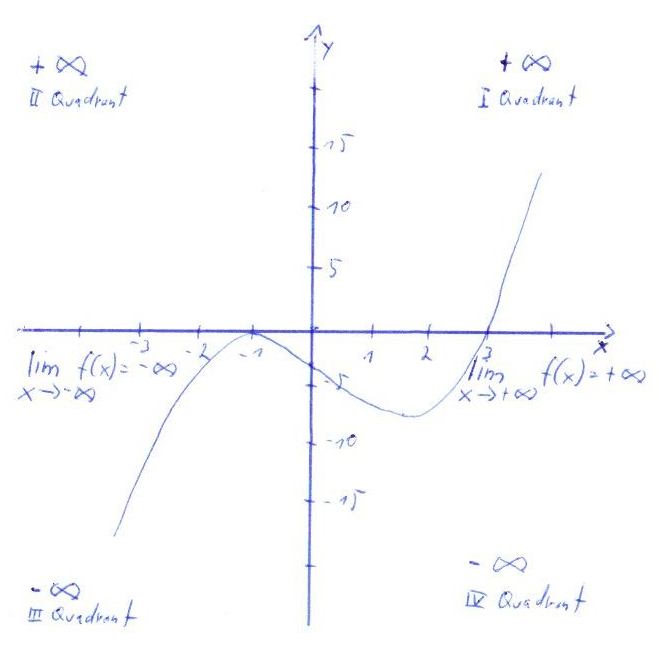
\includegraphics[width=0.8\textwidth]{5c.png}
\end{figure}	
	
As we can see, the graph goes up towards $\infty$ and goes down towards $-\infty$. 	
	
	
	\item Find $f'$ and $f''$.\\
	\textbf{Solutions:}
	
\begin{align}
	f(x) = (x+1)^2(x-3) = (x+1)(x+1)(x-3) = x^3 - x^2 - 5x - 3\notag
\end{align}		
	
\begin{align}
	f'(x) &= 3x^2 - 2x - 5\notag\\
	f''(x) &= 6x - 2\notag
\end{align}	
\vspace{1em}	
	
	\item Find the zeros of $f'$ and $f''$.\\
	\textbf{Solution:}
	
\begin{align}
	3x^2 - 2x - 5 = 0\notag
\end{align}		
	
Apply abc-formula:

\begin{align}
	x &= \frac{2 \pm \sqrt{(-2)^2 - 4 \cdot 3 \cdot (-5)}}{6}\notag\\
	&= \frac{2 \pm \sqrt{64}}{6}\notag\\
	&= \frac{2 \pm 8}{6}\notag\\
	x_1 &= -1\notag\\ 
	x_2 &= \frac{5}{3}\notag
\end{align}	
	
Zeros of $f'$ = $\{-1,\frac{5}{3}\}$\\

\begin{align}
	6x - 2 &= 0\notag\\
	6x &= 2\notag\\
	x &= \frac{1}{3}\notag
\end{align}	
	
Zeros of $f''(x) = \frac{1}{3}$\\	
	
	\item What are the critical points (determine their $x$ and $y$ coordinates)?\\
	\textbf{Solution:}\\
	
A critical point of a function $f: D \rightarrow \mathbb{R}$, is a point $a \in D$ such that $f'(a) = 0$. The value $f(a)$ is called a critical value of f.\\


Determine critical points by plugging in the values where $f'(x) = 0$ into the original function\\



\begin{align*}
	(-1)^3 - (-1)^2 - 5(-1) - 3 &= -1 -1 +5 -3\notag\\
	&= 0
\end{align*}
	
Critical point 1: $(-1,0)$\\

\begin{align*}
	(\frac{5}{3})^3 - (\frac{5}{3})^2 - 5(\frac{5}{3}) - 3 &= \frac{125}{27} - \frac{25}{9} - 5\frac{25}{3} - 3\notag\\
	&= \frac{125}{27} - \frac{75}{27} - \frac{225}{27} - 3\notag\\
	&= -\frac{256}{27}
\end{align*}

Critical point 2: $(\frac{5}{3},-\frac{256}{27})$\\	
	
	\item Find the local minima and maxima.\\
	\textbf{Solution:}\\

When a function's slope is zero at $x$, and the second derivative at $x$ is:

\begin{itemize}
	\item less than 0, it is a local maximum
	\item greater than 0, it is a local minimum
	\item equal to 0, then the test failes
\end{itemize}

Plugging-in the zeros of $f'$ into $f''(x)$:\\

\begin{align*}
	6(-1) -2 = -8\notag\\
\end{align*}

Therefore, $(-1,0)$ is a local maximum.\\

\begin{align*}
	6(\frac{5}{3}) -2 = 8\notag\\
\end{align*}

Therefore, $(\frac{5}{3},-\frac{256}{27})$ is a local minimum.\\

	
	\item Which parts of the function are convex and concave? Does function $f$ have points of inflection? (Hint: Use the sign of the second derivative for anwering both questions.)\\
	\textbf{Solution:}\\	
	
A \textbf{point of inflection} on a curve $y = f(x)$ is a point at which $f$ changes from concave to convex or vice versa.	
	
\begin{itemize}
	\item If $f''(x) > 0$, for all $x \in (a,b)$, then $f$ is convex on $(a,b)$
	\item If $f''(x) < 0$, for all $x \in (a,b)$, then $f$ is concave on $(a,b)$
	\item If $f$ has an inflection point at x and $f''$ exists in $(x - \delta, x + \delta)$, for some $\delta > 0$, then $f''(x) = 0$
\end{itemize}	

Calculating points of inflection:

\begin{align*}
f''(x) &= 0\notag\\
6x - 2 &= 0\notag\\
x &= \frac{1}{3}\notag
\end{align*}
				
\begin{align*}
	f'''(x) &= 6 \notag\\
	f'''(\frac{1}{3}) > 0 &\rightarrow \text{change from concave to convex}
\end{align*}		
\end{enumerate}

Calculating point of inflection by plugging in $\frac{1}{3}$ into $f$:\\

\begin{align*}
f(\frac{1}{3}) &= \frac{1}{3}^3 - \frac{1}{3}^2 - \frac{5}{3} - 3\notag\\
 &= \frac{1}{27} - \frac{1}{9} - \frac{5}{3} - 3\notag\\
 &= -4\frac{20}{27}
\end{align*}

Point of inflection: $\left( \frac{1}{3}, -4\frac{20}{27} \right)$

We know the local minima/maxima, behaviour towards $\infty$ and $-\infty$ and the point of inflection by now. Therefore, we can divide the function into the parts we want to inspect with regards to their convexity and concavity:

\begin{itemize}
	\item $(- \infty, -1)$, $f''(-2) = -14 \rightarrow \text{concave}$
	\item $(-1, \frac{1}{3})$, $f''(0) = -2 \rightarrow \text{concave}$
	\item $\frac{1}{3},\frac{5}{3}$, $f''(\frac{2}{3}) = 2 \rightarrow \text{convex}$
	\item $(\frac{5}{3}, \infty)$, $f''(2) = 10 \rightarrow \text{convex}$
\end{itemize}



\item (\textbf{25 points}) We will investigate the function

\begin{align}
	f(x) = \frac{(x-2)^2}{x+2}\notag
\end{align}

following similar steps at the ones in the previous problem. Additionally, we prove that the line $y = x - 6$ is a slant asymptote on both sides

\begin{enumerate}
	\item Determine the domain of function $f$.\\
	\textbf{Solution:}
		
\begin{align}
	D(f) = \{ x \in \mathbb{R} | x \neq -2 \}\notag
\end{align}
\vspace{1em}		
		
		
	\item What are the roots of $f$? Where does the graph of $f$ intersect the $y$ axsis?\\
	\textbf{Solution:}\\
	
To get the roots of $f$ (x-intercepts) which is a quotient in that case, we just have to set the numerator to zero.\\

Therefore, the root is $2$.\\
We could also expand the numerator to $x^2 - 4x + 4$ and then apply the abc-formula, but that's kind of an overkill in this case.\\

To get the y-intercept, we just have to plug-in 0:

\begin{align}
	f(x) &= \frac{(x-2)^2}{x+2}\notag\\
	f(0) &= \frac{(0-2)^2}{0+2}\notag\\
	&= 2\notag
\end{align}	
	
Y-intercept at 2.\\
	
	
	
	
	\item Determine the limits at the edges of the domain. In this case, there are only two edges:
	
	\begin{align}
	\lim_{x \to -\infty }f(x) \qquad and \qquad \lim_{x \to +\infty}f(x)\notag	
	\end{align}	
	\textbf{Solution}:\\
	

	
\begin{align}
	\lim_{x \to -\infty} \frac{x^2 - 4x + 4}{x+2} &= \frac{\lim_{x \to -\infty}x^2 - 4x + 4 }{\lim_{x \to -\infty} x + 2} \notag\\
	&= \frac{\infty}{-\infty}\notag\\
	&= \text{undefined expression}\notag
\end{align}	
	
Therefore, we have to apply L'Hopital's rule. 	
	
\begin{align*}
\frac{d}{dx} x^2 - 4x + 4 = 2x - 4\notag\\
\frac{d}{dx} x + 2 = 1\notag\\
\end{align*}

\begin{align}
	\lim_{x \to -\infty} \frac{2x - 4}{1} &= -\infty\notag 
\end{align}	

The same procedure can be applied for $\lim_{x \to \infty} \frac{x^2 - 4x + 4}{x+2}$
	
\begin{align}
	\lim_{x \to \infty} \frac{2x - 4}{1} &= \infty\notag 
\end{align}		
	
	\item Find $f'$ and $f''$.\\
	\textbf{Solutions:}\\
	
\begin{align}
	f(x) &= \frac{(x-2)^2}{x+2}\notag\\
	&= \frac{x^2 - 4x + 4}{x+2}\notag
\end{align}	
	
\begin{align}
	f'(x) &=  \frac{\left[ (2x - 4)(x+2))\right] - \left[ (x^2 - 4x +4) \cdot 1\right]}{(x+2)^2}\notag\\
	&= \frac{x^2 - 4x - 12}{(x+2)^2}\notag\\
	&= \frac{(x-2)(x+6)}{(x+2)^2}\notag\\
	&= \frac{x^2 + 4x - 12}{(x+2)^2}\notag
\end{align}


\begin{align}
	f''(x) &= \frac{\left[(2x+4)(x+2)^2\right] - \left[ (x^2-4x-12)(2x+4)\right]}{(x+2)^4}\notag\\
	&= \frac{32}{(x+2)^3}\notag
\end{align}

	
	
	\item Find the zeros of $f'$ and $f''$.\\
	\textbf{Solution:}\\
	
Zeros of $f'(x) = \{ 2,-6\}$. Known by the products in the numerator.\\

Zeros of $f''(x)$ are undetermined.\\	
	
	
	
	\item What are the critical points (determine their $x$ and $y$ coordinates)?\\
	\textbf{Solution:}\\
	
	
A critical point of a function $f: D \rightarrow \mathbb{R}$, is a point $a \in D$ such that $f'(a) = 0$. The value $f(a)$ is called a critical value of f.\\


Determine critical points by plugging in the values where $f'(x) = 0$ into the original function\\



\begin{align*}
	\frac{(2 - 2)^2}{2+2} = 0\notag\\
\end{align*}
	
Critical point 1: $(2,0)$\\

\begin{align*}
	\frac{(-6 - 2)^2}{-6+2} &= \frac{64}{-4}\notag\\
	&= -16\notag
\end{align*}

Critical point 2: $(-6,-16)$\\		
	
	
	
	
	\item Find the local minima and maxima.\\
	\textbf{Solution:}\\

When a function's slope is zero at $x$, and the second derivative at $x$ is:

\begin{itemize}
	\item less than 0, it is a local maximum
	\item greater than 0, it is a local minimum
	\item equal to 0, then the test failes
\end{itemize}

Plugging-in the zeros of $f'$ into $f''(x)$:\\

\begin{align*}
	\frac{32}{(2+2)^3} = \frac{1}{2}\notag\\
\end{align*}

Therefore, $(2,0)$ is a local minimum.\\

\begin{align*}
	\frac{32}{(-6+2)^3} = -\frac{1}{2}\notag\\
\end{align*}

Therefore, $(-6,-16)$ is a local maximum.\\


	
	
	\item Which parts of the function are convex and concave? Does function $f$ have points of inflection? (Hint: Use the sign of the second derivative for anwering both questions.)\\
	\textbf{Solution:}\\	
	
$f''(x) = 0$ is undetermined. Therefore, there is no point of inflection.	
	
	\item Show that the line $y = x - 6$ is a slant asymptote of f. (Hint: use the definition on slide 47 of the lecture and the following two limits.)
	
	\begin{align}
		\lim_{x \ to -\infty}(f(x) - (x-6)) = ? \quad and \quad \lim_{x \to +\infty}(f(x) - (x-6)) = ?\notag
	\end{align}		
\textbf{Solution:}\\	
	
	
\end{enumerate}


\item (\textbf{10 points}) Misc

\begin{enumerate}
	\item Find the derivative of $f(x) = \ln(\cos(\ln(\cos(x)))).$\\
	\textbf{Solution:}\\
	
	
\begin{align}
	f'(x) &= \frac{1}{\cos(\ln(\cos(x)))} \cdot (-\sin(\ln(\cos(x)))) \cdot \frac{1}{\cos(x)} \cdot (-\sin(x))\notag\\
	&= \frac{-\sin(\ln(\cos(x)))}{\cos(\ln(\cos(x)))} \cdot \frac{-\sin(x)}{\cos(x)}\notag\\
	&= -\tan(\ln(\cos(x))) \cdot (-\tan(x))\notag
\end{align}	
	
	
	
	\item Find a function $g(x)$ such that $g'(x) = \tan(2x).$\\
	\textbf{Solution:}
	
\begin{align*}
	g(x) &= -\frac{1}{2}\ln(\cos(2x)) + c\notag
\end{align*}	
\vspace{1em}		
	
	
	\item Find three functions $f_1, f_2, f_3$ such that $f'_1(x) = f'_2(x) = f'_3(x) = \sin(x)\cos(x)$.\\
	\textbf{Solution:}\\
		
	
\end{enumerate}




\end{enumerate}

\end{document}
